%
High-performance computing resources play a key role in advancing computational science by enabling modeling of scientific phenomena at high spatiotemporal resolutions.
%
%Although HPC enables modeling of scientific phenomena at high spatiotemporal resolutions, the total data generated is prohibitively large.
%
A challenge with regard to studying the output of a simulation is the prohibitively large size of the total data generated.
%
Compromise in the form of storing a subset of the data can impact the extent and accuracy of subsequent post hoc exploratory analysis and visualization.
%
In particular, for accurate time-varying vector field analysis and visualization, access to the full spatiotemporal resolution is required.
%
Since storing the entire simulation output is expensive, scientists resort to temporal subsampling or lossy compression, and often limit analysis to individual time slices.
%
An emerging paradigm to address large data challenges is the use of in situ processing to perform runtime analysis/visualization or data reduction to support exploratory post hoc analysis.
%
%

%
Lagrangian analysis is a powerful tool to study time-varying vector fields and is widely employed for ocean modeling applications~\cite{VANSEBILLE201849}.
%
The notion of calculating a Lagrangian representation or \textit{flow map}, i.e., sets of particle trajectories, ``online'' (in situ) for ``offline'' (post hoc) exploration was first proposed by Vries et al.~\cite{vries2001calculating} for an ocean modeling simulation.
%
Figure~\ref{fig:sample} illustrates the approach.
%
More recently, multiple works have advanced Lagrangian research along axes such as strategies for in situ extraction of reduced Lagrangian representations~\cite{agranovsky2014improved}\cite{rapp2019void}\cite{sane2020scalable}, post hoc reconstruction~\cite{chandler2015interpolation}\cite{sane2019interpolation}\cite{Jakob20}, and theoretical error analysis~\cite{bujack2015lagrangian}\cite{chandler2016analysis}\cite{hummel2016error}.
%

An open challenge for time-varying vector field exploration is predicting the uncertainty and variability in accuracy for different analysis techniques.
%
Although the effectiveness of Lagrangian representations for any possible time-varying vector field that can be produced by a scientific simulation remains an open question, prior theoretical demonstration of Lagrangian techniques~\cite{agranovsky2014improved}\cite{chandler2015interpolation}\cite{bujack2015lagrangian}\cite{chandler2016analysis}\cite{hummel2016error}\cite{sane2018revisiting}\cite{sane2019interpolation}\cite{rapp2019void}\cite{Jakob20} on analytical, SPH, climate and ocean modeling data, and practical application in ocean activity analysis~\cite{envirvis.20171099}\cite{siegfried2019tropical}, has provided encouraging results.
%
Using Lagrangian representations, the quality of post hoc reconstruction depends on the vector field itself, as well as configuration specifics such as sampling strategy and frequency of storage.
%
Thus, to investigate the potential benefits of Lagrangian representations for a broader range of applications and to gauge its viability in practice, we leverage the recent developments of runtime in situ infrastructure that enable the straightforward extraction via APIs to study Lagrangian representations for cosmology and seisomology applications.   

\begin{figure}[!t]
\centering
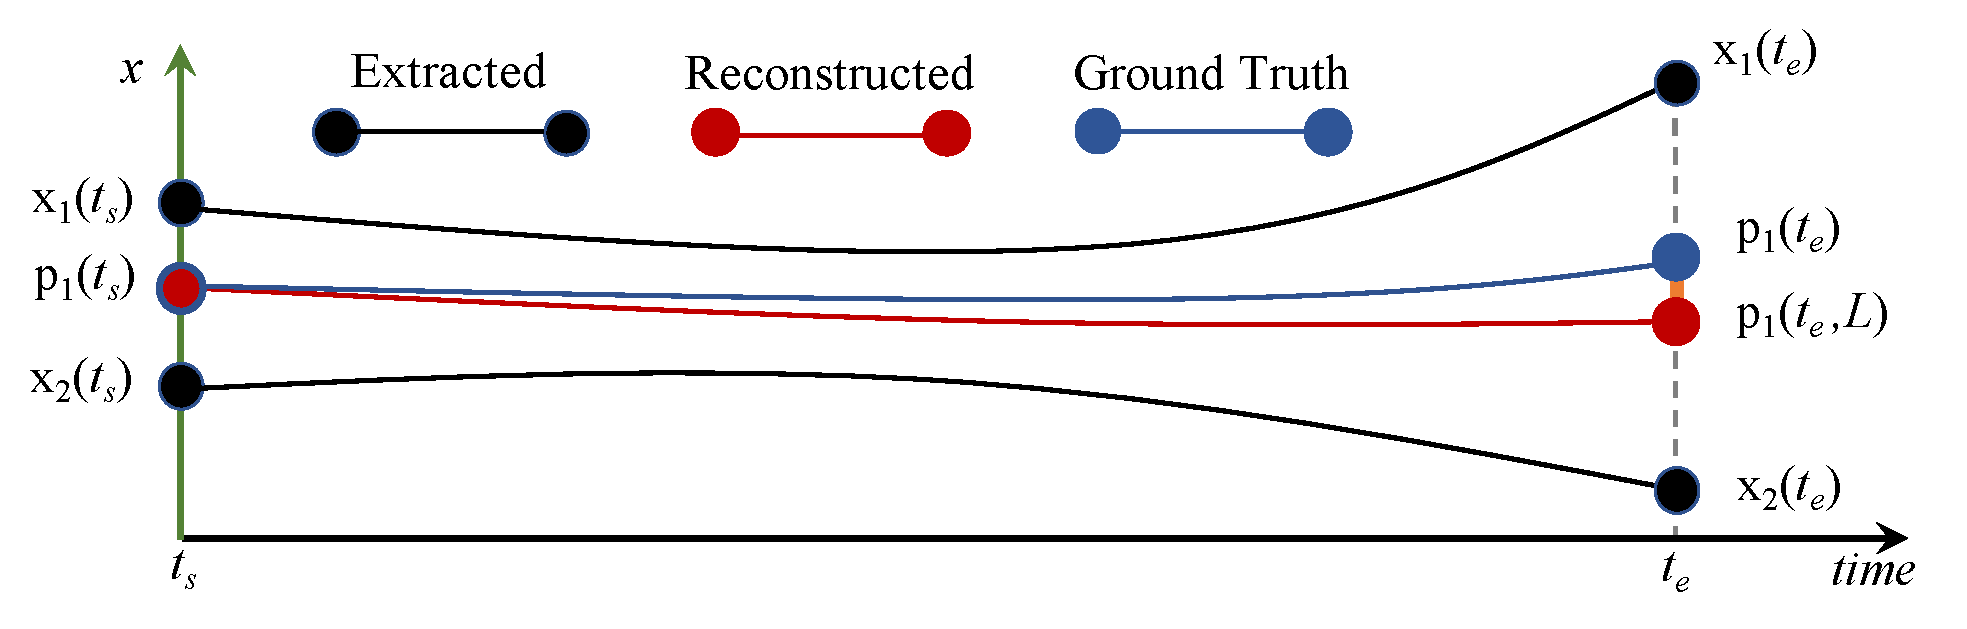
\includegraphics[width=0.85\linewidth]{Images/sample.pdf}
\vspace{-3mm}
\caption{Notional space-time visualization of Lagrangian representations for a time-varying 1D flow. The black trajectories are computed in situ and encode the behavior of the vector field between start time \textit{t$_{s}$} and end time \textit{t$_{e}$}. In a post hoc setting, a Lagrangian-based advection scheme \textit{L}, i.e., a technique to interpolate the extracted data, is used to calculate the trajectory of a new particle p$_{1}$ . The red trajectory is the trajectory reconstructed post hoc and the blue trajectory is the ground truth. The end location of the red trajectory deviates by a margin of error from the ground truth.}
%The quality of reconstruction often depends on the nature of the time-varying vector field.}
\vspace{-8mm}
\label{fig:sample}
\end{figure}

In this paper, our unique contribution is an investigation of Lagrangian representations to encode self-gravitating gas dynamics of a cosmology simulation and seismic wave propagation of a seisomology simulation.
%
We measure the effectiveness of the technique by considering in situ encumbrance and post hoc accuracy.
%
For both applications, our experiments show that Lagrangian representations offer high data reduction, in many cases requiring less than 1\% storage of the complete time-varying vector fields, for a small loss of accuracy. 
%
Further, our study shows Lagrangian representations are viable to compute in representative HPC environments, requiring under 10\% of total execution time for data analysis and visualization in the majority of configurations tested. 
